\begin{figure}[!htb]
    \centering
    \resizebox{15.5cm}{!}{
    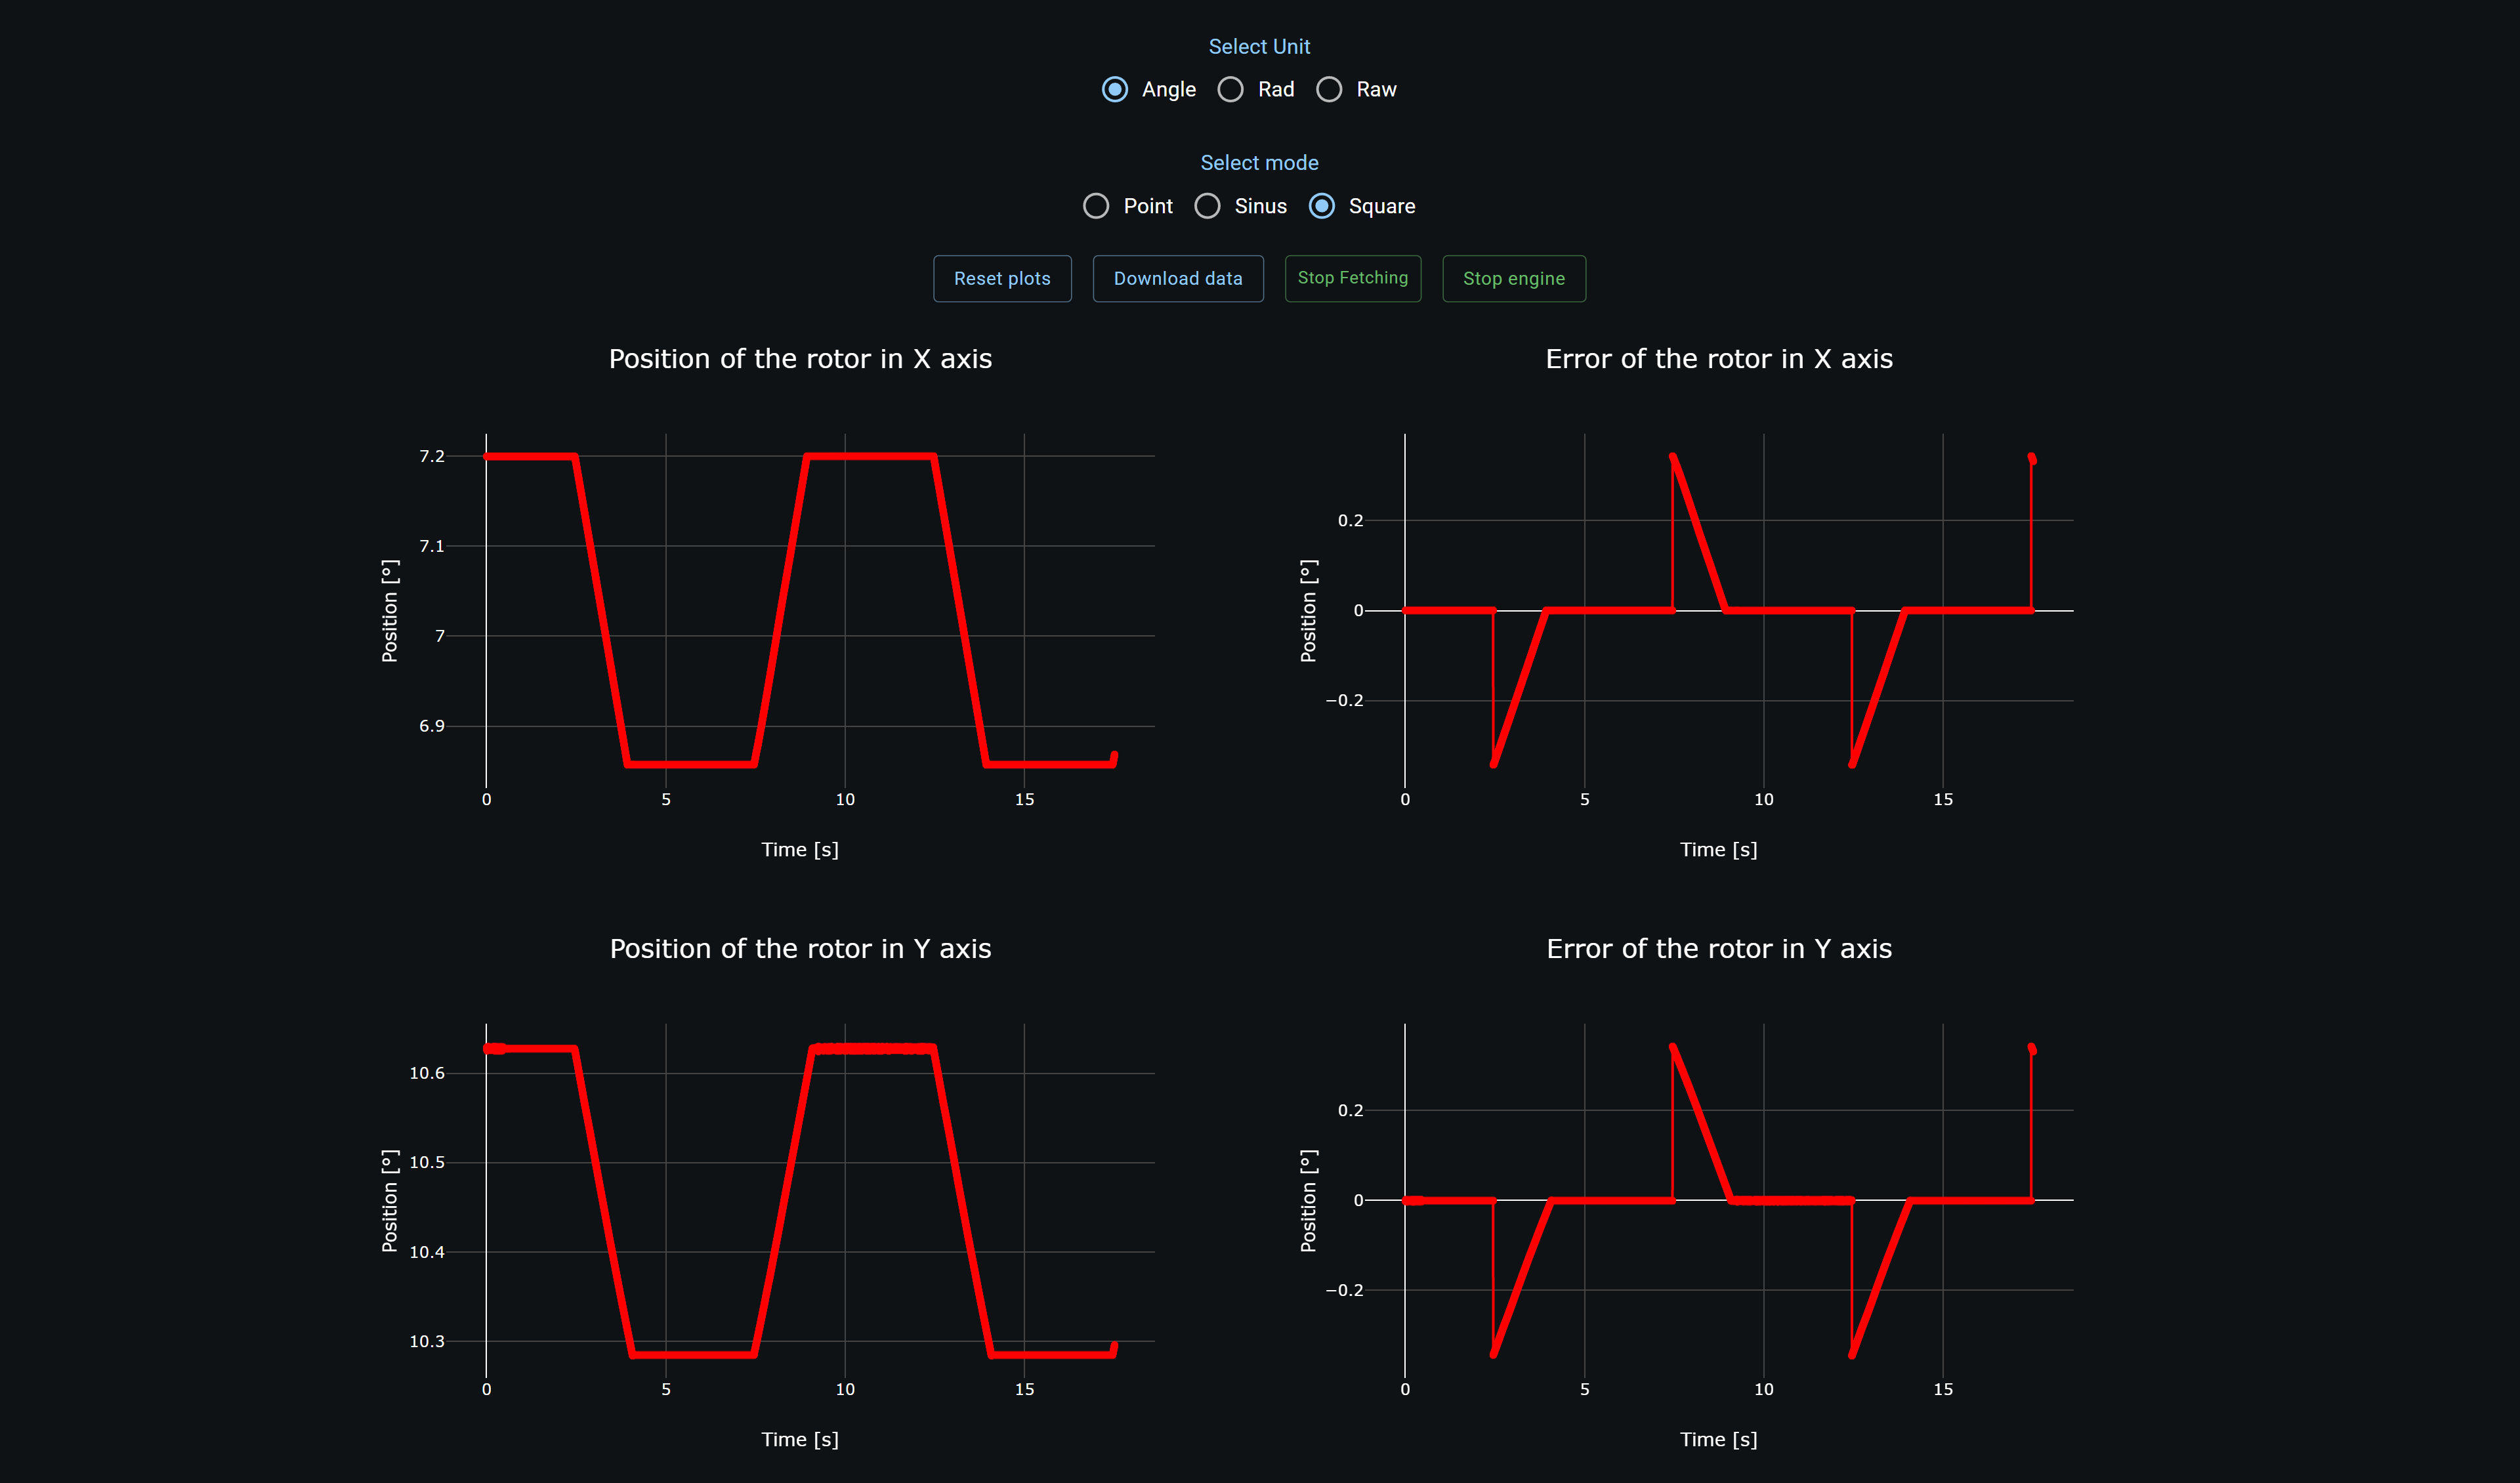
\includegraphics{interface/aplikacja webowa.png}}
    \label{fig:Interfejs}
    \caption{Interfejs użytkownika}
\end{figure}
\section{Funkcja wyboru jednostki}
\begin{enumerate}
    \item \textbf{Angle:} pozycja w stopniach.
    \item \textbf{Rad:} pozycja w radianach.
    \item \textbf{Raw:} pozycja odczytana przez enkoder.
\end{enumerate}
Wybranie jednostki powoduje zmianę wartości na osi rzędnych wykresów. Dodatkowo podczas wpisywania pozycji brana jest wybrana jednostka np. przy wybraniu \textbf{Raw} wpisujemy wartość np. \textit{20000000}, natomiast przy wybraniu \textbf{Rad} wpisujemy np. \textit{0.12} w celu ustawienia pozycji.
\section{Wybranie trybu wartości zadanej}
\begin{enumerate}
    \item \textbf{Point:} pokazuje interfejs z polami tekstowymi, które umożliwiają wpisanie wartości zadanej.
    \item \textbf{Sinus:} ustawia trajektorie sinusoidalną.
    \item \textbf{Square:} ustawia trajektorie prostokątną.
\end{enumerate}
W przypadku wybrania trybu \textbf{Sinus} lub \textbf{Square} interfejs z inputami do wpisywania wartości zadanej jak i przycisk \textbf{Send message} jest chowany.
\section{Przyciski funkcyjne}
\begin{enumerate}
    \item \textbf{Reset plots:} usuwa aktualne próbki w pamięci, również czyści wykresy.
    \item \textbf{Download data:} pobiera aktualne próbki w formacie JSON, struktura jest taka sama jak JSON przesyłany z STM32 do aplikacji webowej.
    \item \textbf{Start Fetching:} aktywuje pobieranie próbek do buforu na STM32. Załącza zegar, który co \textit{200ms} pobiera próbki z STM32 próbki i wyświetlane na wykresach. Po pobraniu próbek bufor na STM32 jest czyszczony. Dodatkowo zmienia nazwę przycisku na "Stop Fetching" i zmienia kolor na zielony.
    \item \textbf{Stop Fetching:} wyłącza zegar odpowiedzialny za pobieranie próbek co 200ms, a następnie zmienia nazwę przycisku na "Start Fetching" i zmienia kolor.
    \item \textbf{Start engine:} aktywuje piny pozwalające na pracę rotorów. Również aktywuje sygnał \textit{CLK} odpowiedzialny za ruch rotorów.
    \item \textbf{Send message:} wpisana pozycja jest przekształcana na jednostkę Raw, a następnie jest przesyłana do STM32. Końcowo STM32 ustawia te pozycje jako wartości zadane.
\end{enumerate}
W polach tekstowych Position X i Position Y należy wpisać wartość zadaną według wybranej jednostki.
\section{Schemat blokowy pobierania danych}
Po wciśnięciu przycisku \textit{Start Fetching} w interfejsie użytkownika załączany jest zegar z okresem \textit{200ms}. Rozpoczyna on cykliczny proces wymiany danych pomiędzy frontendem, backendem jak i mikrokontrolerem. Szczegółowy opis komunikacji:

\begin{enumerate}
    \item \textbf{Frontend:} inicjuje wysyłanie zapytań w formacie JSON do backendu za pomocą protokołu WebSocket. Każda wiadomość zawiera klucz \textbf{isFetching} o wartości \textit{1}. 
    \item \textbf{Backend:} przesyła otrzymaną wiadomość do serwera na mikrokontrolerze.
    \item \textbf{Serwer na mikrokontrolerze:}  Po otrzymaniu klucza \textbf{isFetching} o wartości \textit{1}, rozpoczyna się zapisywanie próbek z aktualną pozycją i uchybem do bufora, o ile zapis nie był wcześniej zainicjowany. Po przetworzeniu danych z backendu, serwer zwraca JSON'a o strukturze zawartej w listingu \ref{lst:json_exampleSTM32}. W przypadku pierwszego zapytania bufor jest pusty, dlatego serwer zacznie zwracać niepuste dane dopiero od drugiego zapytania. Po przesłaniu danych bufor z aktualną pozycją i uchybem jest czyszczony.
    \item \textbf{Powrót danych z serwera:} Backend otrzymuje wiadomość w fragmentach i składa ją w całość. Każdy fragment jest dodawany do buforu. W przypadku gdy cała wiadomość jest w buforze, czyli zawiera znak końca JSON "\textbf{\{}", wysyła ją do frontendu za pomocą protokołu WebSocket, a po jej wysłaniu usuwa ją z buforu. W przypadku braku pełnej wiadomości backend oczekuje na kolejne fragmenty. Frontend, po otrzymaniu wiadomości, aktualizuje wykresy, dodając nowe próbki o aktualnej pozycji i uchybie.
    \item \textbf{Zatrzymanie procesu:} Proces powtarza się co \textit{200ms}, dopóki użytkownik nie naciśnie przycisku \textit{Stop Fetching}. Po jego aktywacji zegar zostanie zatrzymany i zostanie wysłana wiadomość z kluczem \textit{isFetching} o wartości \textit{0}, co skutkuje zatrzymaniem zapisywania aktualnych próbek do buforu na mikrokontolerze.
\end{enumerate}
Na Rys. ~\ref{fig:schemat blokowy pobierania danych} przedstawiono proces wymiany danych między frontendem, backendem aplikacji webowej i serwerem na mikrokontrolerze.
 \begin{figure}[H]
    \centering
    \resizebox{15.5cm}{!}{
    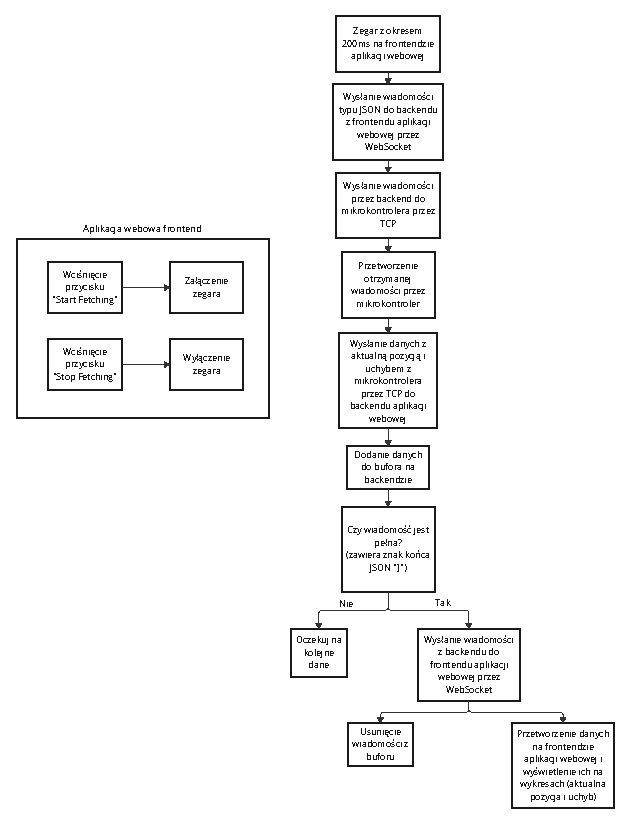
\includegraphics{interface/schemat blokowy pobierania danych.pdf}}
    \caption{Schemat blokowy pobierania pozycji i uchybu.}
    \label{fig:schemat blokowy pobierania danych}
\end{figure}
\section{Docker}
Docker \cite{Docker} jest narzędziem do konteneryzacji, które umożliwia tworzenie i uruchamianie aplikacji w kontenerach, czyli odizolowanych środowiskach. Kontenery są instancjami obrazów Dockera, które dzięki swojej zoptymalizowanej budowie cechują się lekkością i możliwością ponownego wykorzystania. Zawierają jedynie niezbędne elementy do prawidłowego działania aplikacji.
\subsection{Działanie Dockera}
Docker polega na zasadzie wirtualizacji na poziomie systemu operacyjnego. Główne narzędzia Dockera:
\begin{enumerate}
    \item \textbf{Obrazy}: są to szablony zawierające system operacyjny i podstawowe zależności do działania aplikacji.
    \item \textbf{Kontenery}:
    Obraz Dockera może zostać uruchomiony jako kontener, który działa w odizolowanym środowisku. Dzięki temu wszyscy mogą pracować w identycznych warunkach, co eliminuje potrzebę tworzenia i konfigurowania środowisk dla każdej osoby z osobna. Ponadto Docker rozwiązuje problem różnic w działaniu aplikacji na różnych systemach operacyjnych, zapewniając spójność i przewidywalność.
\end{enumerate}

\subsection{Zalety Dockera}
\begin{enumerate}
    \item \textbf{Przenośność}: Kontenery mogą być uruchamiane na różnych systemach operacyjnych i infrastrukturach, co ułatwia wdrażanie aplikacji.
    Docker może zostać użyty na głównych systemach operacyjnych, co znacząco ułatwia wdrażanie aplikacji. Mac i linux posiadają paczki do instalacji dockera, natomiast na windowsie można użyć aplikacji docker deskop i dodatkowo zainstalować podsystem linux WSL2 (Windows subsystem for linux), w celu zwiększenia wydajności kontenerów.
    \item \textbf{Izolacja}:
    Aplikacja działa w odizolowanym środowisku, co minimalizuje konflikty między środowiskami i zależnościami.
    \item \textbf{Szybkość}:
    Kontenery są lekkie i szybkie do uruchomienia w porównaniu do maszyn wirtualnych. Kontenery używają tylko najpotrzebniejszych zależności, co przyczynia się do ich lekkości.
    \item \textbf{Skalowalność}: Docker umożliwia w prosty sposób skalowanie aplikacji, poprzez uruchamianie wielu kontenerów jednocześnie. Np. na jednym kontenerze mamy aplikację webową, a na drugim można byłoby dodać bazę danych.
\end{enumerate}
\subsection{Obraz i kontener użyty w aplikacji}
Przy budowaniu obrazu został rozszerzony obraz \textit{node:22-alpine}, \textit{alpine} oznacza okrojoną wersję, która posiada tylko najpotrzebniejsze zależności. Na tym obrazie dostępny jest Node.js w wersji 22. Dodatkowo został zainstalowany bash, który ułatwia poruszanie się po zbudowanym kontenerze. Do zbudowania obrazu zostały użyte polecenia instalujące paczki NPM potrzebne do prawidłowego działania aplikacji, dodatkowo instalowana jest globalnie paczka serve, która służy do obsługi serwera HTTP. Po włączeniu kontenera inicjowane są polecenia uruchamiające WebSocket na porcie \textbf{8080} jak i aplikacje webową, przy użyciu serwera HTTP, na porcie \textbf{3000}. Powyższe porty są udostępniane kontenerowi za pomocą polecenia \textit{EXPOSE}. W pliku konfiguracyjnym kontenera zdefiniowano również porty hosta, które są dostępne z poziomu komputera. Porty hosta mogą być takie same jak w kontenerze, ale istnieje możliwość ich zmiany, co pozwala na mapowanie różnych portów na potrzeby specyficznych konfiguracji i unikanie konfliktów. Nazwa kontenera została ustawiona na app\_container. Dodatkowo została udostępniona sieć dla kontenera, w celu prawidłowego połączenia się z serwerem na STM32.
\subsection{Uruchomienie aplikacji w kontenerze}
Całą aplikację można uruchomić poleceniem \textit{docker compose up}. Po użyciu tej komendy na porcie \textbf{3000} jest dostępna aplikacja z intefejsem do obsługi teleskopu i WebSocket na porcie \textbf{8080}. W celu wejścia na kontener należy użyć polecenia \textit{docker exec -it app\_container bash}.